\section{Importing/exporting data)}

{\setbeamercolor{background canvas}{bg=LemonChiffon}
\begin{frame}
\frametitle{}
{\fontsize{40}{50}\selectfont Programming in Python \#1} 

{\huge importing/exporting data} 

\end{frame}
}

\begin{frame}
\frametitle{}

\huge \textit{El més important, que quedi clar el zen de python}

\end{frame}




%--------------------------------------------------------------------------------------------------------------
\begin{frame}
\frametitle{Objective}

Be able to read/write data in various formats used in oceanography

\vfill 

\onslide<2->{
Text files (ascii)\\
CSV\\
NetCDF\\
HDF\\
Images (geotiff)\\
matlab files\\
\ldots
}
\vfill 
\onslide<3->{Be able to find the resources to read another format}

\end{frame}

%--------------------------------------------------------------------------------------------------------------
\subsection{ipython notebook}
%--------------------------------------------------------------------------------------------------------------

\begin{frame}[c]
\frametitle{What is an ipython notebook?}


\begin{description}
\item<2->[Python:] high-level programming language\\ 
\url{https://www.python.org/}
\item<3->[IPython:] command shell for interactive computing\\ 
\url{http://ipython.org/}
\item<4->[IPython notebook:] web-based interactive computational environment combining code, text, figures, \ldots\\
\url{http://ipython.org/notebook.html}
\end{description}

\end{frame}

%--------------------------------------------------------------------------------------

\begin{frame}[c]
\footnotesize
\frametitle{Why ipython notebooks?}


\includegraphics[width=2.5cm]{ipython_logo}

\vspace{1cm}

\begin{itemize}
\item User-friendly
\item Free, easy to write, easy to read
\item Code and results visible online via \url{http://nbviewer.ipython.org}
\item[]
\item<2-> \textit{Data story-telling}
\end{itemize}

\end{frame}

%--------------------------------------------------------------------------------------------------------------

\begin{frame}
\frametitle{Structure of a notebook}

\begin{columns}[c]

\begin{column}{.8\linewidth}
\begin{tikzpicture}
    \node[anchor=south west,inner sep=0] (image) at (0,0) {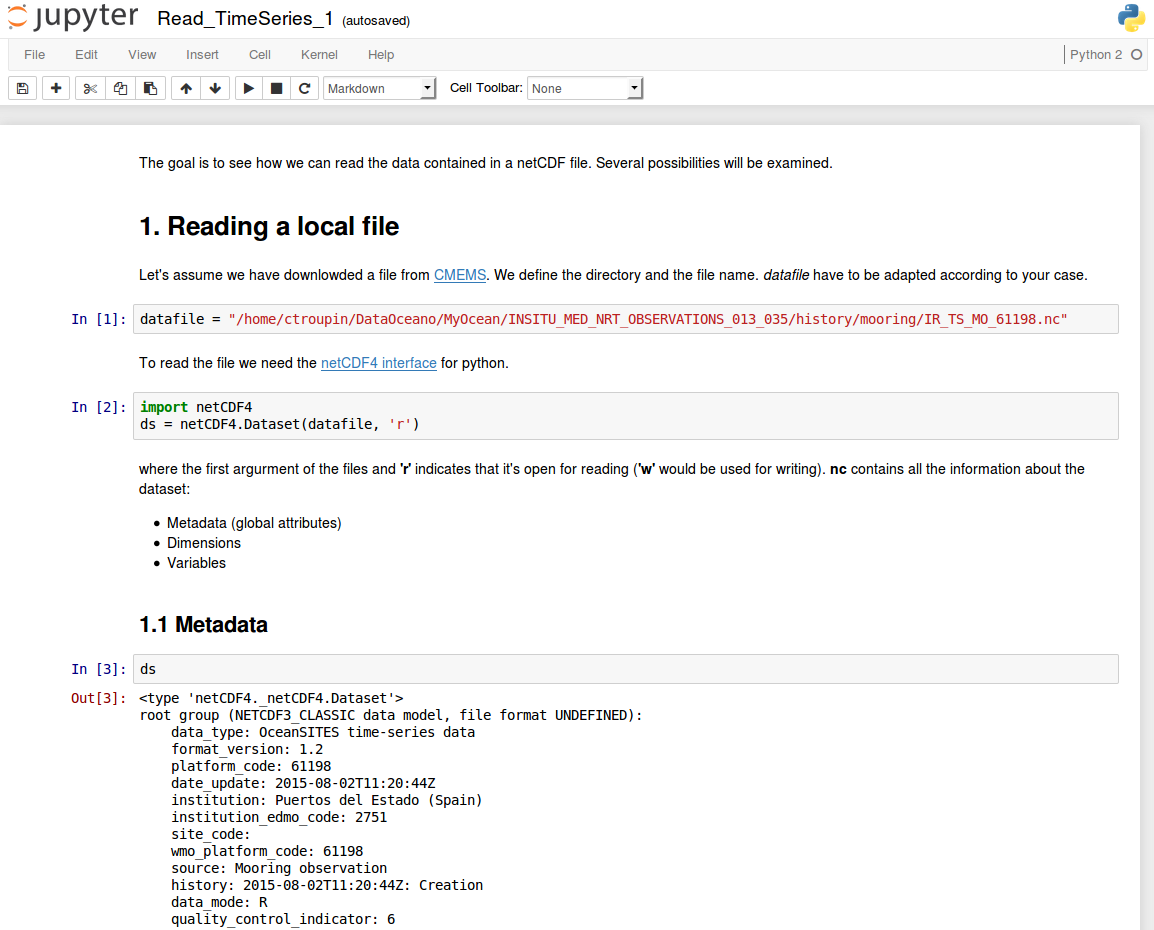
\includegraphics[width=.95\textwidth]{notebook_insitu1}};
    \begin{scope}[x={(image.south east)},y={(image.north west)}]
		\path (.21,.9) coordinate (play1);
		\path (.05,.9) coordinate (add1);
		\path (.35,.9) coordinate (cell1);
		\path (.05,.65) coordinate (code1);
		\path (.11,.49) coordinate (text1);
%		\draw[help lines,xstep=.1,ystep=.1] (0,0) grid (1,1);
%		\foreach \x in {0,1,...,9} { \node [anchor=north] at (\x/10,0) {0.\x}; }
%		\foreach \y in {0,1,...,9} { \node [anchor=east] at (0,\y/10) {0.\y}; }
    \end{scope}  
     
\end{tikzpicture}

\end{column}


\begin{column}{.2\linewidth}

\scriptsize 
\onslide<2->{\tikz[na] \coordinate (play2); Run current cell}

\onslide<3->{\tikz[na] \coordinate (add2); Add a new cell}

\onslide<4->{\tikz[na] \coordinate (cell2); Select type of cell}

\onslide<5->{\tikz[na] \coordinate (code2); Code cell}

\onslide<6>{\tikz[na] \coordinate (text2); Text cell}

\end{column}

\end{columns}

\begin{tikzpicture}[overlay]
\begin{scope}[x={(image.south east)},y={(image.north west)}]
	\onslide<2>{\path[*-stealth,arrowcolor,thin,opacity=0.25] (play1) edge [out=-90, in=180] (play2);}
	\onslide<3>{\path[*-stealth,arrowcolor,thin,opacity=0.25] (add1) edge [out=-90, in=180] (add2);}
	\onslide<4>{\path[*-stealth,arrowcolor,thin,opacity=0.25] (cell1) edge [out=-90, in=180] (cell2);}
	\onslide<5>{\path[*-stealth,arrowcolor,thin,opacity=0.25] (code1) edge [out=0, in=180] (code2);}
	\onslide<6>{\path[*-stealth,arrowcolor,thin,opacity=0.25] (text1) edge [out=0, in=180] (text2);}
\end{scope}
\end{tikzpicture}

\end{frame}



%--------------------------------------------------------------------------------------------------------------
\subsection{Comma-Separated Values file}
%--------------------------------------------------------------------------------------------------------------
\begin{frame}[fragile]
\frametitle{Comma-Separated Values file}

\begin{onlyenv}<1>
Example: file \pyfile{buoy-canaldeibiza\_SALT\_SBE37.csv}

\begin{lstlisting}[language=bash,basicstyle=\tiny,title={Example of CSV file}]
Platform, Instrument, Paramenter, Units, Date, Value, QC value 
Buoy_CanalDeIbiza, SCB-SBE37006, sea_water_salinity, psu, 2015-12-01 12:00:00, 36.916, 1.0
Buoy_CanalDeIbiza, SCB-SBE37006, sea_water_salinity, psu, 2015-12-01 01:00:00, 36.936, 1.0
Buoy_CanalDeIbiza, SCB-SBE37006, sea_water_salinity, psu, 2015-12-01 02:00:00, 36.929, 1.0
Buoy_CanalDeIbiza, SCB-SBE37006, sea_water_salinity, psu, 2015-12-01 03:00:00, 36.927, 1.0
Buoy_CanalDeIbiza, SCB-SBE37006, sea_water_salinity, psu, 2015-12-01 04:00:00, 36.925, 1.0
Buoy_CanalDeIbiza, SCB-SBE37006, sea_water_salinity, psu, 2015-12-01 05:00:00, 36.948, 1.0
Buoy_CanalDeIbiza, SCB-SBE37006, sea_water_salinity, psu, 2015-12-01 06:00:00, 36.95, 1.0
Buoy_CanalDeIbiza, SCB-SBE37006, sea_water_salinity, psu, 2015-12-01 07:00:00, 36.954, 1.0
Buoy_CanalDeIbiza, SCB-SBE37006, sea_water_salinity, psu, 2015-12-01 08:00:00, 36.933, 1.0
\end{lstlisting}
\end{onlyenv}

\begin{itemize}
\item<2-> Type "python read csv file" in search engine
\item<3-> Result: \url{https://docs.python.org/2/library/csv.html}\\
\item<4-> From the doc:
\begin{lstlisting}[language=python,basicstyle=\tiny]
import csv
csvfile = open('buoy-canaldeibiza\_SALT_SBE37.csv', 'rb')
reader = csv.reader(csvfile)
for row in reader:
  print row
csvfile.close()
\end{lstlisting}
\end{itemize}

\vfill

\begin{onlyenv}<5>
\notebook \verb|read_csv_file.ipynb|
\end{onlyenv}
\end{frame}

%--------------------------------------------------------------------------------------------------------------
\subsection{CNV file}
%--------------------------------------------------------------------------------------------------------------

\begin{frame}[fragile]
\frametitle{Seabird CTD file}

\begin{onlyenv}<1>
Example: file \pyfile{dsb01.cnv}

\begin{lstlisting}[language=bash,basicstyle=\tiny,title={Example of CNV file}]
* Sea-Bird SBE 9 Data File:
* FileName = C:\OCEANO\CTD\DATOS\IMEDEA-SHEBEX\SB01.hex
* Software Version Seasave V 7.22
* Temperature SN = 5427
* Conductivity SN = 3872
...
38.86539  2.78989  ... 3.4535e-02    7.459    
38.86542  2.78986  ... 223 0.0000e+00
\end{lstlisting}
\end{onlyenv}

\begin{itemize}
\item<2-7> Type "python read cnv file" in search engine
\item<3-7> Result: \url{https://pypi.python.org/pypi/cnv}\\
{\tiny\it "Sorry for the inconvenience, but I moved all the functionalities into the package seabird"}
\item<4-7> Use pip to search for the package
\begin{lstlisting}[language=bash,basicstyle=\tiny]
pip search seabird
seabird     - Non official parser for Sea-Bird's sensors.
\end{lstlisting}
\item<5-7> Install package:
\begin{lstlisting}[language=bash,basicstyle=\tiny]
pip install --user seabird==0.6.3
\end{lstlisting}
\item<6-7> From the doc:
\begin{lstlisting}[language=python,basicstyle=\tiny]
from seabird.cnv import fCNV
profile = fCNV('')
profile.attributes 	# It will return the header, as a dictionary.
profile.keys()		# It will list the available variables.
profile['TEMP']   	# Get the data
\end{lstlisting}
\end{itemize}

\vfill 
\begin{onlyenv}<7>
\notebook \verb|read_cnv_file.ipynb|
\end{onlyenv}

\end{frame}


%--------------------------------------------------------------------------------------------------------------

%\begin{frame}[fragile]
%\frametitle{Seabird CTD file: example}
%
%\begin{onlyenv}<1>
%Open file:
%\begin{lstlisting}[language=python,basicstyle=\tiny]
%profile = fCNV('dsb01.cnv')
%DEBUG:root:Openning file: dsb01.cnv
%DEBUG:root:Using rules from: cnv.yaml
%\end{lstlisting}
%\end{onlyenv}
%
%\begin{onlyenv}<2>
%Check attributes:
%\begin{lstlisting}[language=python,basicstyle=\tiny]
%In [15]: profile.attributes
%Out[15]: 
%{'LATITUDE': 38.86516666666667,
% 'LONGITUDE': 2.79,
% 'bad_flag': '-9.990e-29',
% 'datetime': datetime.datetime(2015, 5, 10, 15, 43, 53),
% 'file_type': 'ascii',
% 'filename': 'dsb01.cnv',
% 'gps_datetime': 'May 10 2015  15:43:53',
% 'instrument_type': 'CTD',
% 'md5': 'e13cc440d147cdb0e9f76c6a1a630d3a',
% 'nquan': '27',
% 'nvalues': '231',
% 'sbe_model': '9',
% 'seasave': 'V 7.22',
% 'start_time': 'May 10 2015 15:43:53 [NMEA time, header]'}
%\end{lstlisting}
%\end{onlyenv}
%
%
%\begin{onlyenv}<3>
%List available variables:
%\begin{lstlisting}[language=python,basicstyle=\tiny]
%In [19]: profile.keys()
%Out[19]: 
%['LATITUDE',
% 'LONGITUDE',
% 'DEPTH',
% 'PRES',
% 'TEMP',
% 'TEMP2',
% 'T2-T190C',
% 'c0mS/cm',
% 'c1mS/cm',
% 'C2-C1mS/cm',
% 'PSAL',
% 'PSAL2',
% 'secS-priS',
% 'density',
% 'density',
% 'D2-D1,d',
% 'sbeox0Mg/L',
% 'spar',
% 'par',
% 'flSP',
% 'seaTurbMtr',
% 'DEPTH',
% 'PSAL',
% 'density',
% 'sigma-\xe900',
% 'nbin',
% 'flag']
%\end{lstlisting}
%\end{onlyenv}
%
%\begin{onlyenv}<4>
%Show temperature:
%\begin{lstlisting}[language=python,basicstyle=\tiny]
%In [20]: profile['TEMP']
%Out[20]: 
%masked_array(data = [19.9946 18.0183 17.1547 16.9913 16.5491 15.4609 15.0954 14.6589 14.3429
% 14.2343 14.0877 13.9795 13.9342 13.9389 13.9535 13.9477 13.9299 13.8918
% ...
% 13.1806 13.1814 13.1821 13.1826 13.1832 13.1841],
%             mask = [False False False False False False False False False False False False
% False False False False False False False False False False False False
% ...
% False False False],
%       fill_value = -9.99e-29)
%\end{lstlisting}
%
%\end{onlyenv}
%
%\end{frame}

\subsection{A few words about github}

\begin{frame}[fragile]
\frametitle{How to get code from github}

\url{https://github.com/ctroupin/PythonCourseCadiz2016}

\begin{tikzpicture}
    \node[anchor=south west,inner sep=0] (image) at (0,0) {\includegraphics[width=.85\textwidth]{pythongithub}};
    \begin{scope}[x={(image.south east)},y={(image.north west)}]
		\path (.9,.6) coordinate (DownloadZIP);
		\path (.7,.6) coordinate (clone);
%		\draw[help lines,xstep=.1,ystep=.1] (0,0) grid (1,1);
%		\foreach \x in {0,1,...,9} { \node [anchor=north] at (\x/10,0) {0.\x}; }
%		\foreach \y in {0,1,...,9} { \node [anchor=east] at (0,\y/10) {0.\y}; }
    \end{scope}  
     
\end{tikzpicture}

\onslide<2->{\tikz[na] \coordinate (DownloadZIP2); Click and download the \texttt{.zip} file or \ldots}

\onslide<3->{\tikz[na] \coordinate (clone2); Copy the URL and type \texttt{git clone url} in a terminal}


\begin{tikzpicture}[overlay]
\begin{scope}[x={(image.south east)},y={(image.north west)}]
	\onslide<2>{\path[*-stealth,arrowcolor,thin,opacity=0.25] (DownloadZIP) edge [out=-90, in=180] (DownloadZIP2);}
	\onslide<3>{\path[*-stealth,arrowcolor,thin,opacity=0.25] (clone) edge [out=-90, in=180] (clone2);}
\end{scope}
\end{tikzpicture}

\end{frame}

\begin{frame}[fragile]
\frametitle{Update the code}

\begin{enumerate}
\item<1-> Clone the repository 

\begin{lstlisting}[language=bash]
git clone https://github.com/... .git
\end{lstlisting}

\item<2-> \faHourglass3 \comment{(if there were modifications in the repository)}

\item<3-> Update your version 

\begin{lstlisting}[language=bash]
git pull 
\end{lstlisting}
\end{enumerate}

\onslide<4->{More about github:
\begin{itemize}
\item \url{https://github.com/}
\item \url{http://rogerdudler.github.io/git-guide/}}
\end{itemize} 
\end{frame}

%--------------------------------------------------------------------------------------------------------------
\subsection{NetCDF file}
%--------------------------------------------------------------------------------------------------------------
\begin{frame}
\frametitle{NetCDF}

\begin{description}
\item<1->[Definition:] software libraries and self-describing, machine-independent data formats (source: \url{http://www.unidata.ucar.edu/software/netcdf/}).
\item<2->[Users:] atmospheric/ocean observing/modelling communities:  NOAA, EUMETSAT, NASA/JPL, USGS, Copernicus Marine Service, \ldots
\item<3->[Tools:] many tools and libraries to inspect, visualise and explore data sets.
\item<4->[Structure:] \begin{itemize}
\item header: dimensions, attributes, variables 
\item data: arrays
\end{itemize}
  
\end{description}

\end{frame}

%--------------------------------------------------------------------------------------------------------------
\subsubsection{Inspection}
%--------------------------------------------------------------------------------------------------------------

\begin{frame}[c, fragile]
\frametitle{Quick inspection: ncdump}

\begin{description}
\item[\homepage] {\scriptsize \url{https://www.unidata.ucar.edu/software/netcdf/docs/netcdf/ncdump.html}}
\item[\tool] text representation of a netCDF dataset (header information, variables, \ldots)
\end{description}

\vfill

\begin{lstlisting}[language=bash,basicstyle=\tiny,title={ncdump applied on a file}]
ncdump -h 20140628_d-OC_CNR-L3-CHL-MedOC3_A_1KM-MED-DT-v02.nc

netcdf \20140628_d-OC_CNR-L3-CHL-MedOC3_A_1KM-MED-DT-v02 {
dimensions:
	time = 1 ;
	lat = 1580 ;
	lon = 3308 ;
variables:
	int time(time) ;
		time:long_name = "reference time" ;
		time:standard_name = "time" ;
		time:axis = "T" ;
		time:calendar = "Gregorian" ;
		time:units = "seconds since 1981-01-01 00:00:00" ;
...
			"SUBSAMP=1\n",
			"OUTMODE=0\n",
			"" ;
}

\end{lstlisting}

\end{frame}

%--------------------------------------------------------------------------------------------------------------
\subsubsection{Visualisation}
%--------------------------------------------------------------------------------------------------------------
\begin{frame}[c, fragile]
\frametitle{Ferret}


\includegraphics[height=.07\paperwidth]{logo_ferret}

\begin{description}
\item[\homepage] {\scriptsize \url{http://www.ferret.noaa.gov/Ferret/}}
\item[\tool] visualization and analysis environment
\end{description}

\vfill

\begin{lstlisting}[language=bash,basicstyle=\tiny,title={Ferret to get basic info on file}]
ctroupin@SCBD046 ~/Desktop $ ferret_c 
 	NOAA/PMEL TMAP
 	FERRET v6.62  
 	Linux(gfortran) 2.6.9-89.0.20.ELsmp - 07/06/13
 	25-Nov-15 12:23     

yes? SET DATA 20140628_d-OC_CNR-L3-CHL-MedOC3_A_1KM-MED-DT-v02.nc 
yes? SHOW DATA
     currently SET data sets:
    1> 20140628_d-OC_CNR-L3-CHL-MedOC3_A_1KM-MED-DT-v02.nc  (default)
 name     title                             I         J         K         L
 CHL      Mediterranean Sea Daily Chlorop  1:3308    1:1580    ...       1:1
 QI       Quality Index of Mediterranean   1:3308    1:1580    ...       1:1
 
yes? 
\end{lstlisting}


\end{frame}

%-----------------------------------------------------------------------------------------------
\begin{frame}[c]
\frametitle{ncview}

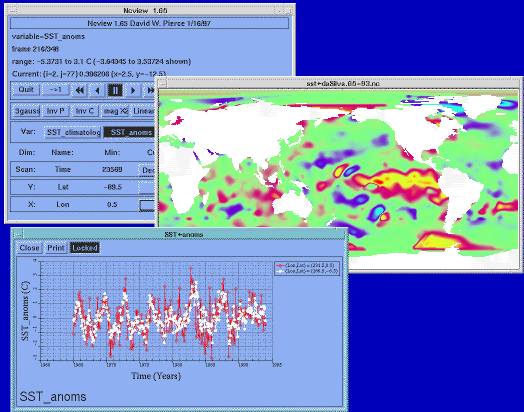
\includegraphics[height=.07\paperwidth]{logo_ncview}

\begin{description}
\item[\homepage] {\scriptsize \url{http://meteora.ucsd.edu/~pierce/ncview_home_page.html}}
\item[\tool] quick visualisation of 3-4D fields
\end{description}

\vfill

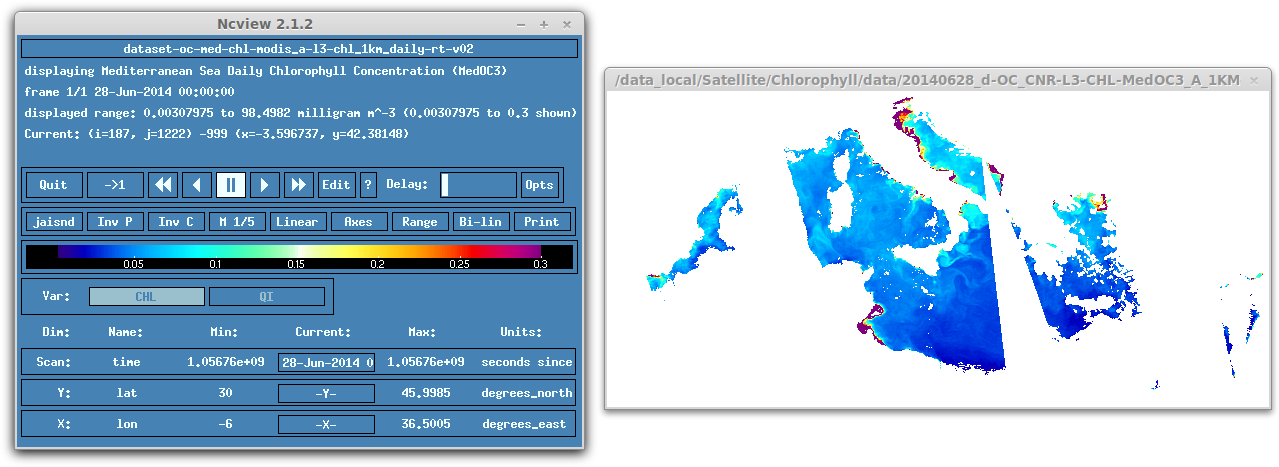
\includegraphics[height=.45\textheight]{ncview1}

\end{frame}

%-----------------------------------------------------------------------------------------------
\begin{frame}[c]
\frametitle{ncbrowse}

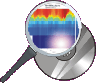
\includegraphics[height=.07\paperwidth]{logo_ncbrowse}

\begin{description}
\item[\homepage] {\scriptsize \url{http://www.epic.noaa.gov/java/ncBrowse/}}
\item[\tool] interactive graphical display
\end{description}

\vfill

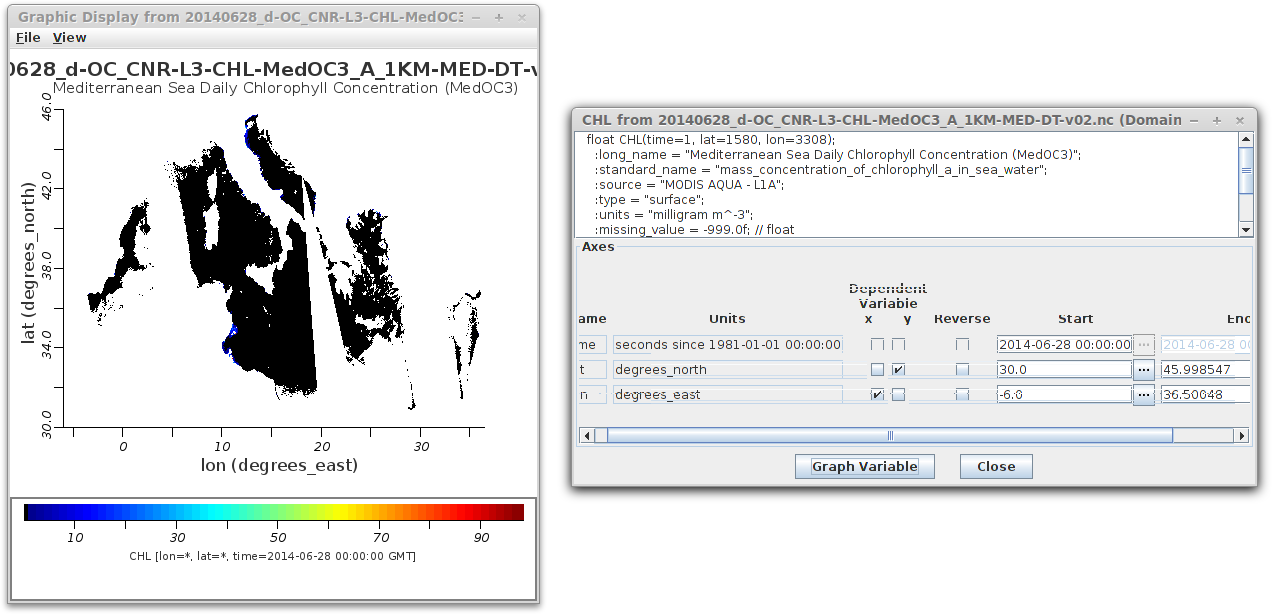
\includegraphics[height=.5\textheight]{ncbrowse1}
\end{frame}

%-----------------------------------------------------------------------------------------------
\begin{frame}[c]
\frametitle{Panoply}

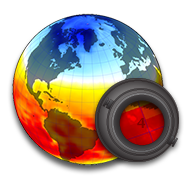
\includegraphics[height=.07\paperwidth]{logo_panoply}

\begin{description}
\item[\homepage] {\scriptsize\url{http://www.giss.nasa.gov/tools/panoply/}}
\item[\tool] plot, slice, combine, overlay, \ldots
\end{description}

\vfill

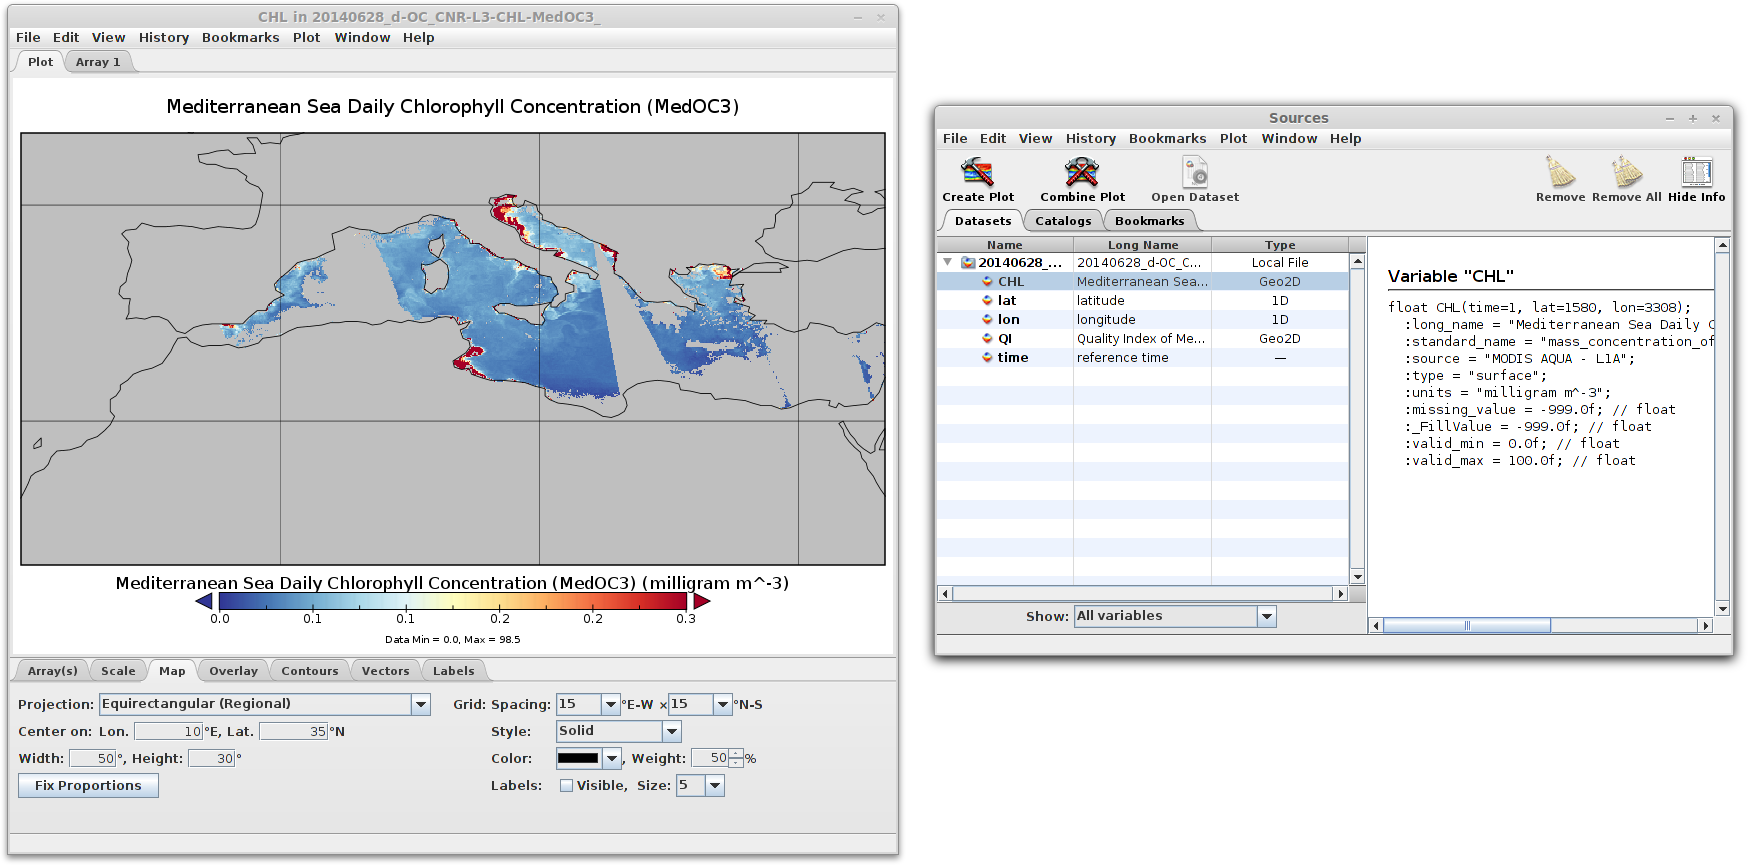
\includegraphics[height=.5\textheight]{panoply1}

\end{frame}

%--------------------------------------------------------------------------------------------------------------
\subsubsection{Processing}
%--------------------------------------------------------------------------------------------------------------

\begin{frame}[c,fragile]
\frametitle{cdo -- Climate Data Operators}


\includegraphics[height=.07\paperwidth]{logo_cdo}

\begin{description}
\item[\homepage] \url{https://code.zmaw.de/projects/cdo}
\item[\tool] manipulate (merging, averaging) netCDF files (+other formats)
\item[Examples:] 
\begin{itemize}
\item Basic info (min, max, avg, size, \ldots):
\begin{lstlisting}[language=bash,basicstyle=\tiny]
cdo info input.nc
\end{lstlisting}
\item Compute standard deviation:
\begin{lstlisting}[language=bash,basicstyle=\tiny]
cdo fldstd input.nc output.nc
\end{lstlisting}
\end{itemize}
\end{description}



\end{frame}
%-----------------------------------------------------------------------------------------------
\begin{frame}[c,fragile]
\frametitle{NCO -- netCDF Operators}


\includegraphics[height=.07\paperwidth]{logo_nco}

\begin{description}
\item[\homepage] \url{http://nco.sourceforge.net/}
\item[\tool] command line operations on netCDF files
\item[Examples:] \begin{itemize}
\item Average variable over domain:
\begin{lstlisting}[language=bash,basicstyle=\tiny]
ncwa -O -a lon,lat input.nc output.nc
\end{lstlisting}
\item Extract subregion:
\begin{lstlisting}[language=bash,basicstyle=\tiny]
ncks -d lon,13.,18.0 -d lat,33.0,36.0 
input.nc output.nc
\end{lstlisting}
\end{itemize}
\end{description}

\end{frame}

%-----------------------------------------------------------------------------------------------
\begin{frame}[c]
\frametitle{ODV -- Ocean Data View}

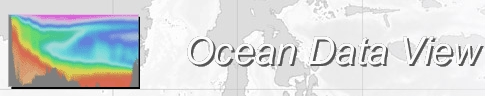
\includegraphics[height=.07\paperwidth]{logo_odv}

\begin{description}
\item[\homepage] \url{http://odv.awi.de/en/home/}
\item[\tool] interactive exploration, analysis and visualization of oceanographic data
\end{description}

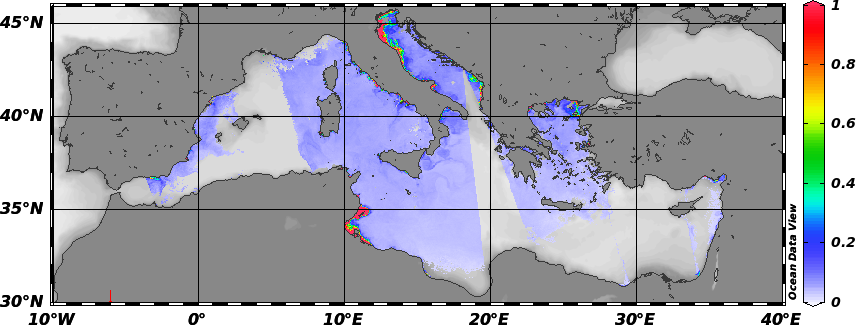
\includegraphics[height=.45\textheight]{odv_chloro1}

\end{frame}

%-----------------------------------------------------------------------------------------------
\begin{frame}[c, fragile]
\frametitle{Octave / Matlab}


\includegraphics[height=.07\paperwidth]{logo_octave}~
\includegraphics[height=.07\paperwidth]{logo_matlab}


High-level functions to read/write data from/to a netCDF file:\\
{\scriptsize
\begin{itemize}
\item \url{http://octave.sourceforge.net/netcdf/overview.html}
\item \url{http://es.mathworks.com/help/matlab/network-common-data-form.html}
\end{itemize}

}
\vfill

\begin{lstlisting}[language=python,basicstyle=\tiny,title=Example with Octave]
nc = netcdf('input.nc','r');             % open netcdf file in read-only
CHL = nc{'CHL'}(:);                      % retrieve variable 
CHL_units = nc{'CHL'}.units;             % retrieve the attribute units
CHL_valid_range = nc{'CHL'}.valid_range; % retrieve the attribute valid_range 
global_history = nc.history;             % retrieve the global attribute history

\end{lstlisting}

\end{frame}

%-----------------------------------------------------------------------------------------------
\begin{frame}[c, fragile]
\frametitle{Python}


\includegraphics[height=.07\paperwidth]{logo_python}

Python interface to the netCDF C library:\\
\url{http://unidata.github.io/netcdf4-python/}

Example: file \pyfile{dep0001\_station-santantoni\_scb-wlog001\_L1\_2016-01.nc}
\vfill

\begin{lstlisting}[language=python,basicstyle=\tiny,title=Example with ipython]
import netCDF4
nc = netCDF4.Dataset('dep0001_station-santantoni_scb-wlog001_L1_2016-01.nc')
print nc
<type 'netCDF4._netCDF4.Dataset'>
root group (NETCDF3_CLASSIC data model, file format UNDEFINED):
    title: Data from instrument SCB-WLOG001 on platform Station SantAntoni
    institution: SOCIB (Sistema de Observacion y prediccion Costero de las Islas Baleares)
    netcdf_version: 3.0
    Conventions: CF-1.6
    abstract: Deployment of instrument SCB-WLOG001 at Sant Antoni station in endurance line

    ...
nc.close()
\end{lstlisting}

\end{frame}


%--------------------------------------------------------------------------------------------------------------
\begin{frame}[c, fragile]
\frametitle{List of notebooks}

Located in \verb|Data_ReadWrite|
{
\scriptsize
\begin{description}
\item[read\_csv\_file.ipynb:] Comma separated values
\item[read\_cnv\_file.ipynb:] SeaBird CTD file
\item[]
\item[read\_netcdf\_local.ipynb:] local \href{http://www.unidata.ucar.edu/software/netcdf/}{netCDF} file
\item[read\_netcdf\_opendap.ipynb:] netCDF on \href{http://www.unidata.ucar.edu/software/thredds/current/tds/}{thredds data server}
\item[read\_netcdf\_cf.ipynb:] netCDF using \href{http://cfconventions.org/}{CF conventions}
\item[read\_shapefile.ipynb:] geospatial vector data
\item[]
\item[read\_geotiff.ipynb:] geotiff image
\item[read\_image.ipynb:] jpg image
\item[]
\item[read\_HDF\_file.ipynb:] Hierarchical Data Format
\item[read\_mat\_file.ipynb:] .mat file


\end{description}
}


\end{frame}

%--------------------------------------------------------------------------------------------------------------
\begin{frame}[c, fragile]
\frametitle{Exercise 1: data reading}

\textbf{Objective:} read \textit{unknown} file format

\vspace{1cm}

\exercise \verb|1-read_CMEMS_indexfile.ipynb|

\end{frame}

